\PassOptionsToPackage{unicode=true}{hyperref} % options for packages loaded elsewhere
\PassOptionsToPackage{hyphens}{url}
%
\documentclass[]{article}
\usepackage{lmodern}
\usepackage{amssymb,amsmath}
\usepackage{ifxetex,ifluatex}
\usepackage{fixltx2e} % provides \textsubscript
\ifnum 0\ifxetex 1\fi\ifluatex 1\fi=0 % if pdftex
  \usepackage[T1]{fontenc}
  \usepackage[utf8]{inputenc}
  \usepackage{textcomp} % provides euro and other symbols
\else % if luatex or xelatex
  \usepackage{unicode-math}
  \defaultfontfeatures{Ligatures=TeX,Scale=MatchLowercase}
\fi
% use upquote if available, for straight quotes in verbatim environments
\IfFileExists{upquote.sty}{\usepackage{upquote}}{}
% use microtype if available
\IfFileExists{microtype.sty}{%
\usepackage[]{microtype}
\UseMicrotypeSet[protrusion]{basicmath} % disable protrusion for tt fonts
}{}
\IfFileExists{parskip.sty}{%
\usepackage{parskip}
}{% else
\setlength{\parindent}{0pt}
\setlength{\parskip}{6pt plus 2pt minus 1pt}
}
\usepackage{hyperref}
\hypersetup{
            pdfborder={0 0 0},
            breaklinks=true}
\urlstyle{same}  % don't use monospace font for urls
\usepackage{graphicx,grffile}
\makeatletter
\def\maxwidth{\ifdim\Gin@nat@width>\linewidth\linewidth\else\Gin@nat@width\fi}
\def\maxheight{\ifdim\Gin@nat@height>\textheight\textheight\else\Gin@nat@height\fi}
\makeatother
% Scale images if necessary, so that they will not overflow the page
% margins by default, and it is still possible to overwrite the defaults
% using explicit options in \includegraphics[width, height, ...]{}
\setkeys{Gin}{width=\maxwidth,height=\maxheight,keepaspectratio}
\setlength{\emergencystretch}{3em}  % prevent overfull lines
\providecommand{\tightlist}{%
  \setlength{\itemsep}{0pt}\setlength{\parskip}{0pt}}
\setcounter{secnumdepth}{0}
% Redefines (sub)paragraphs to behave more like sections
\ifx\paragraph\undefined\else
\let\oldparagraph\paragraph
\renewcommand{\paragraph}[1]{\oldparagraph{#1}\mbox{}}
\fi
\ifx\subparagraph\undefined\else
\let\oldsubparagraph\subparagraph
\renewcommand{\subparagraph}[1]{\oldsubparagraph{#1}\mbox{}}
\fi

% set default figure placement to htbp
\makeatletter
\def\fps@figure{htbp}
\makeatother


\date{}

\begin{document}

\hypertarget{questions}{%
\section{Questions}\label{questions}}

\hypertarget{one}{%
\subsection{One}\label{one}}

\hypertarget{lewis-structure-of-sioh_4}{%
\subsubsection{\texorpdfstring{Lewis structure of
\(Si(OH)_4\)}{Lewis structure of Si(OH)\_4}}\label{lewis-structure-of-sioh_4}}

,\_

\hypertarget{step-1}{%
\paragraph{Step \#1}\label{step-1}}

Number of electrons = 4x6 +4x1 +1x4 = 32.

\hypertarget{step-2}{%
\paragraph{Step \#2}\label{step-2}}

After 8 electrons are assigned to each oxygen, and single bonds are
formed between each species all species have a full octet.

NOTE: As silica is a period two element overfilling of the octet is
possible however any additional bond formation between the oxygen and
the central silicon could only increase the formal charge and so may be
discounted.

\hypertarget{step-3}{%
\paragraph{Step \#3}\label{step-3}}

Draw structure
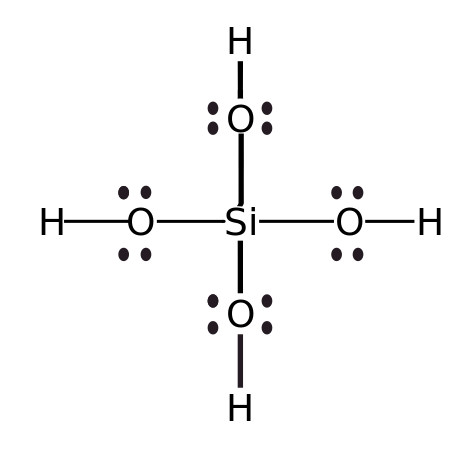
\includegraphics[width=0.5\textwidth,height=\textheight]{Images/SiliconHydroxideLewisStructure.jpg}

\hypertarget{lewis-structure-of-aloh_4--}{%
\subsubsection{\texorpdfstring{Lewis structure of
\(Al(OH)_4 ^{-}\)}{Lewis structure of Al(OH)\_4 \^{}\{-\}}}\label{lewis-structure-of-aloh_4--}}

,\_

\hypertarget{step-1-1}{%
\paragraph{Step \#1}\label{step-1-1}}

Number of electrons = 4x6 +4x1 +1x3+1 = 32.

\hypertarget{step-2-1}{%
\paragraph{Step \#2}\label{step-2-1}}

After 8 electrons are assigned to each oxygen, and single bonds are
formed between each species all species have a full octet. Again
overfilling by creating more bonds will only increase the formal charge.

\hypertarget{step-3-1}{%
\paragraph{Step \#3}\label{step-3-1}}

Draw Structure

\hypertarget{introduction}{%
\section{Introduction}\label{introduction}}

\hypertarget{results}{%
\section{Results}\label{results}}

\end{document}
